\documentclass[a4paper]{article}
\usepackage[margin=1in]{geometry}
\usepackage[english]{babel}
\usepackage[utf8]{inputenc}
\usepackage{amsmath}
\usepackage{graphicx}
\usepackage{booktabs}
% \usepackage[colorinlistoftodos]{todonotes}
\usepackage{setspace}
\doublespacing

\title{CAPP 30254: Assignment 2 Write-up}

\author{Daniel Roberts}

\date{\today}

\begin{document}
\maketitle
\section{Goal}

In this exercise, we attempt to predict the likelihood of serious loan delinquency given a series borrower characteristics. The goal of this exercise was to import, describe, visualize, and clean a dataset of borrower data with loan delinquency status on which we could build a predictive model, then predict values for a set of borrowers for which the actual loan delinquency was unknown.
\section{Statistics}
\par
First, we have a table of summary statistics for the training dataset. Standard deviation is indicated by "std". The median is indicated by "50\%".
\par

\begin{tabular}{lllllllllllll}
\hline
{} & Unnamed: 0 & SeriousDlqin2yrs & RevolvingUtilizationOfUnsecuredLines &  age  \\
\hline
count          &     150000 &           150000 &                               150000 &   150000  \\
mean           &    75000.5 &          0.06684 &                              6.04844 &  52.2952 \\
std            &    43301.4 &         0.249746 &                              249.755 &  14.7719 \\
min            &          1 &                0 &                                    0 &        0 \\
25\%            &    37500.8 &                0 &                            0.0298674 &       41  \\
50\%            &    75000.5 &                0 &                             0.154181 &       52 \\
75\%            &     112500 &                0 &                             0.559046 &       63  \\
max            &     150000 &                1 &                                50708 &      109  \\
missing values &          0 &                0 &                                    0 &        0  \\
\hline
\end{tabular}

\begin{tabular}{lllllllllllll}
\hline
{} & NumberOfTime30-59DaysPastDueNotWorse & DebtRatio & MonthlyIncome \\
\hline
count  & 150000 &    150000 &        120269  \\
mean    &                             0.421033 &   353.005 &       6670.22  \\
std            &                                  4.19278 &   2037.82 &       14384.7  \\
min     &                                    0 &         0 &             0 \\
25\%      &                                    0 &  0.175074 &          3400  \\
50\%          &                                    0 &  0.366508 &          5400 \\
75\%    &                                    0 &  0.868254 &          8249 \\
max    &                                   98 &    329664 &   3.00875e+06  \\
missing values &                                      0 &         0 &         29731 \\
\hline
\end{tabular}

\begin{tabular}{lllllllllllll}
\hline
{} & NumOfOpenCreditLinesAndLoans & NumOfTimes90DaysLate & NumRealEstLoansOrLines  \\
\hline
count  &    150000 &                  150000 &                       150000                           \\
mean    &                            8.45276 &                0.265973 &                      1.01824 \\
std  &                         5.14595 &                  4.1693 &                      1.12977 \\
min     &                               0 &                       0 &                            0 \\
25\%     &                               5 &                       0 &                            0  \\
50\%     &                               8 &                       0 &                            1  \\
75\%     &                              11 &                       0 &                            2  \\
max     &                              58 &                      98 &                           54 \\
missing values  &                               0 &                       0 &                            0\\
\hline
\end{tabular}

\begin{tabular}{lllllllllllll}
\hline
{} & NumberOfTime60-89DaysPastDueNotWorse & NumberOfDependents \\
\hline
count  &                                150000 &             146076 \\
mean   &                             0.240387 &           0.757222 \\
std &                              4.15518 &            1.11509 \\
min    &                                    0 &                  0 \\
25\%    &                                                                0 &                  0 \\
50\%    &                                    0 &                  0 \\
75\%     &                                    0 &                  1 \\
max    &                                   98 &                 20 \\
missing values   &                                    0 &               3924 \\
\hline
\end{tabular}
\newpage
\section{Histograms}
\par  
Below are a series of histograms indicating the distributions of numeric variables in the training dataset.
\begin{center}
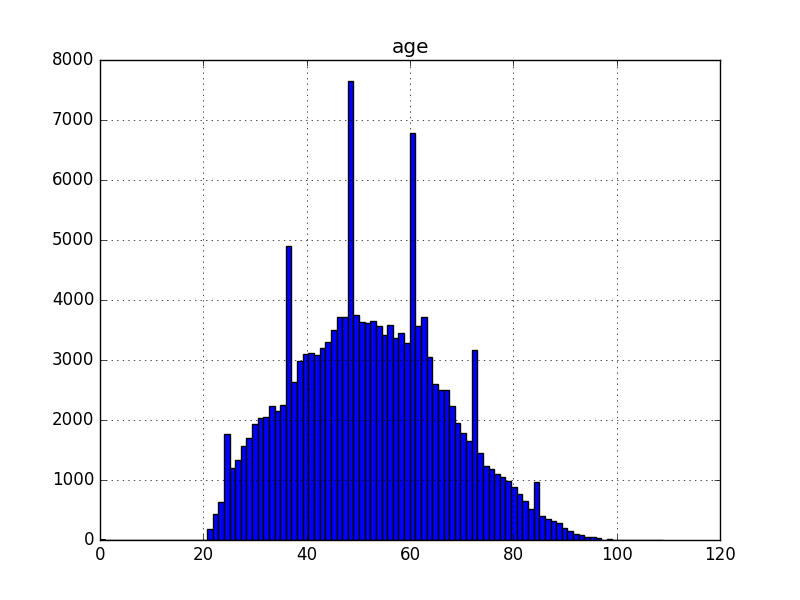
\includegraphics[width=.7\textwidth]{../graphics/train_set_age.png}
\\
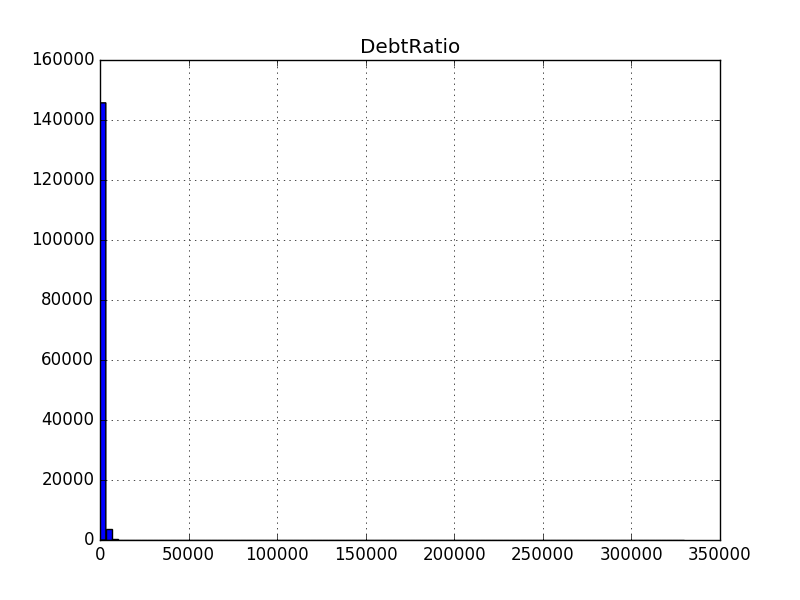
\includegraphics[width=.7\textwidth]{../graphics/train_set_DebtRatio.png}
\\
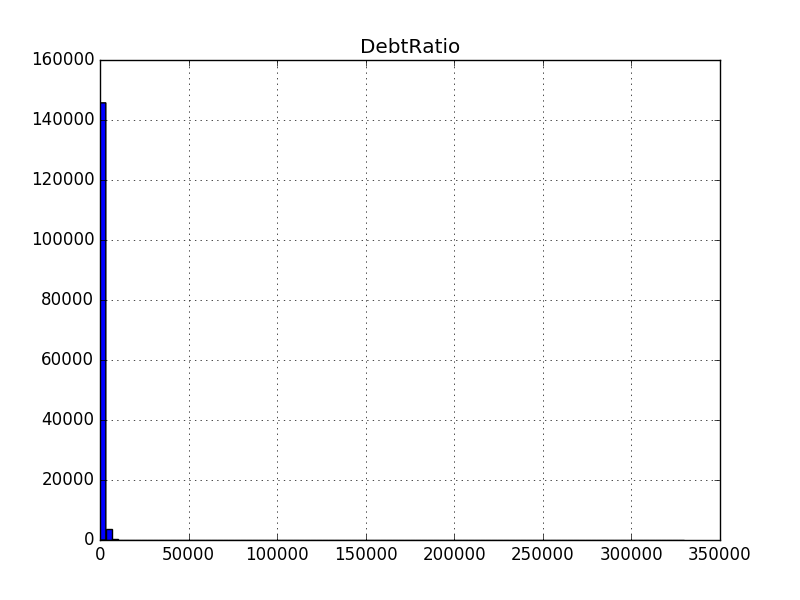
\includegraphics[width=.7\textwidth]{../graphics/train_set_DebtRatio.png}
\\
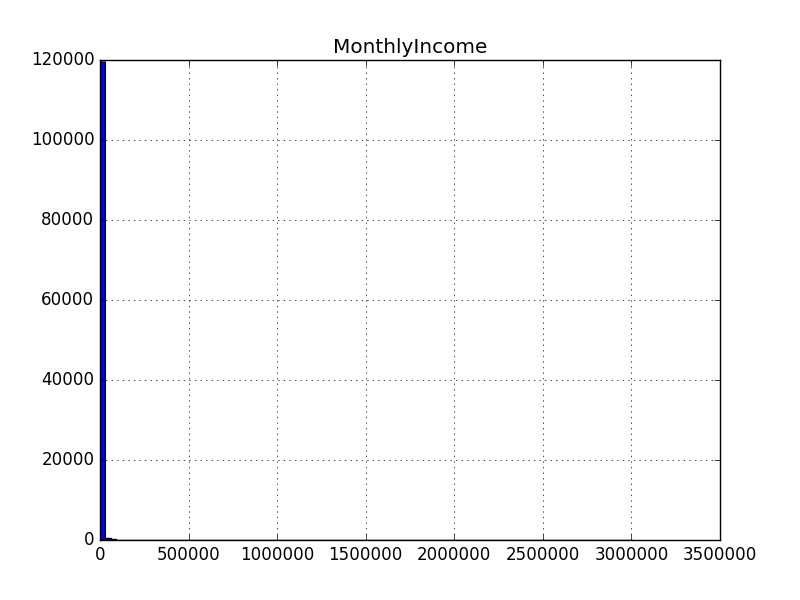
\includegraphics[width=.7\textwidth]{../graphics/train_set_MonthlyIncome.png}
\\
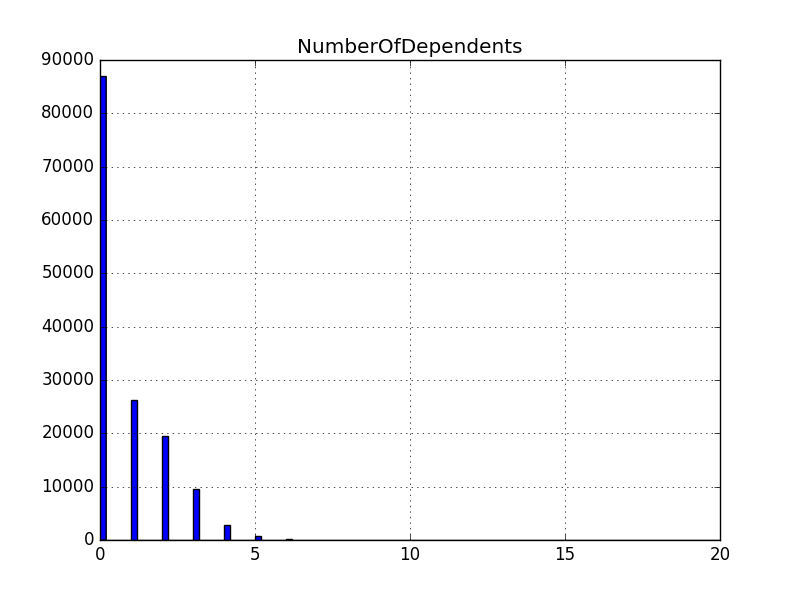
\includegraphics[width=.7\textwidth]{../graphics/train_set_NumberOfDependents.png}
\\
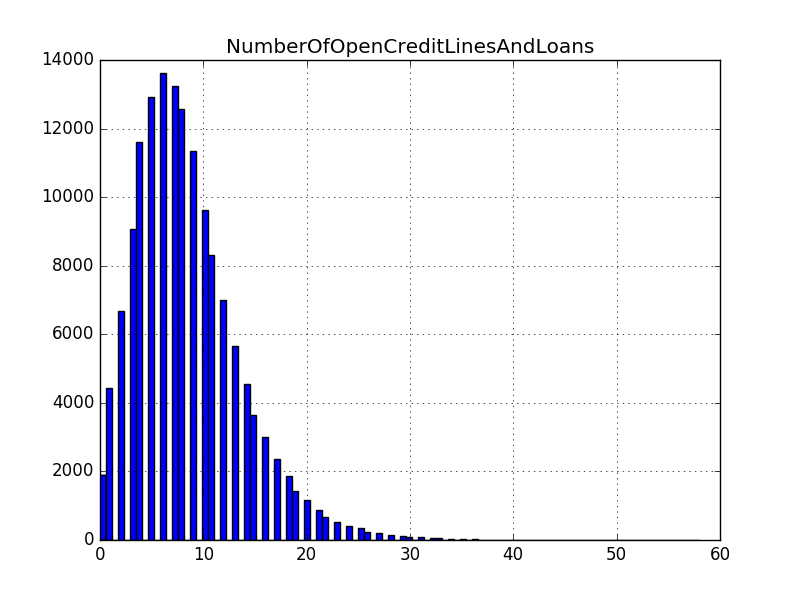
\includegraphics[width=.7\textwidth]{../graphics/train_set_NumberOfOpenCreditLinesAndLoans.png}
\\
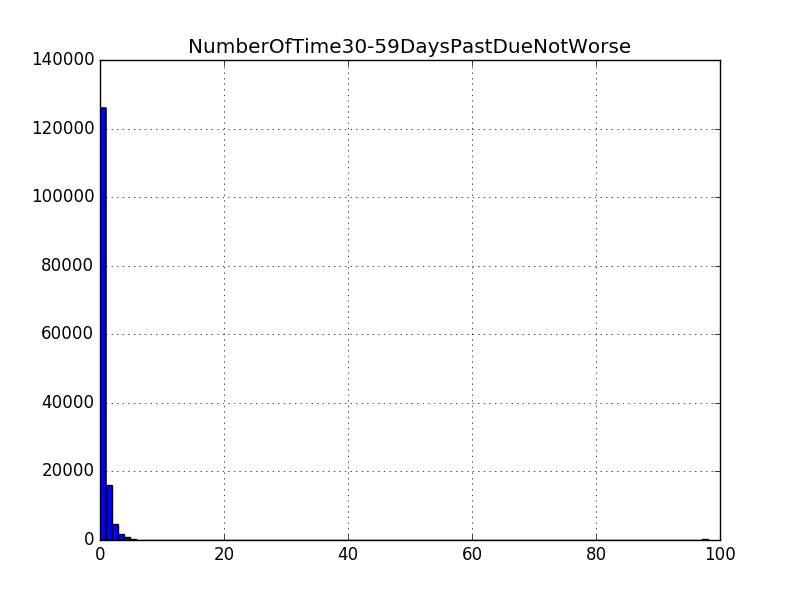
\includegraphics[width=.7\textwidth]{../graphics/train_set_NumberOfTime30-59DaysPastDueNotWorse.png}
\\
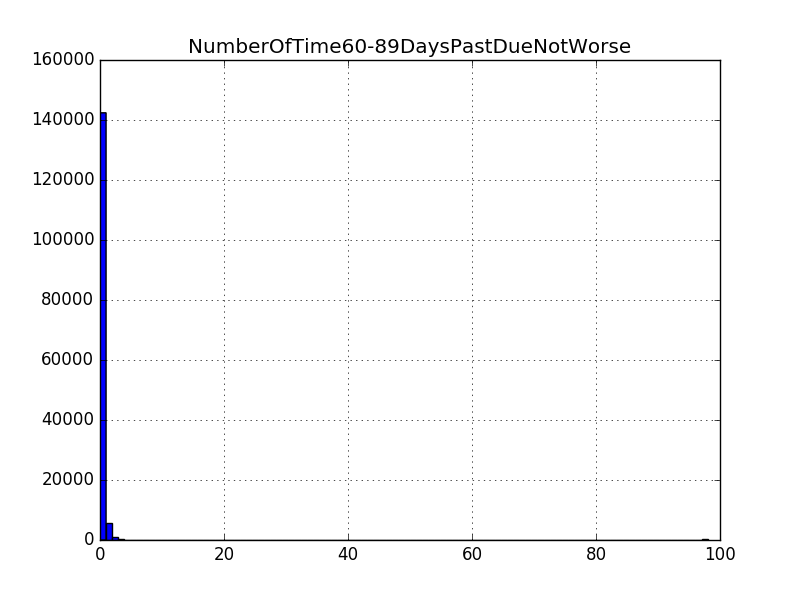
\includegraphics[width=.7\textwidth]{../graphics/train_set_NumberOfTime60-89DaysPastDueNotWorse.png}
\\
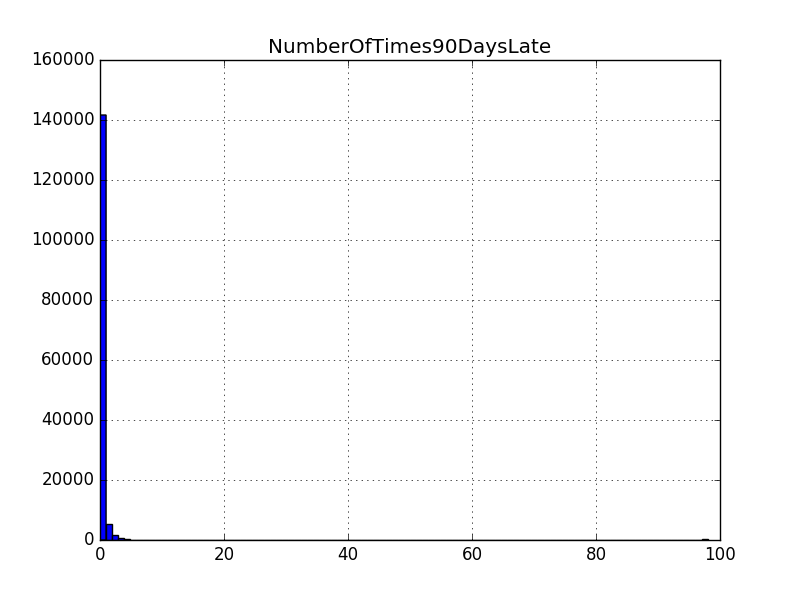
\includegraphics[width=.7\textwidth]{../graphics/train_set_NumberOfTimes90DaysLate.png}
\\
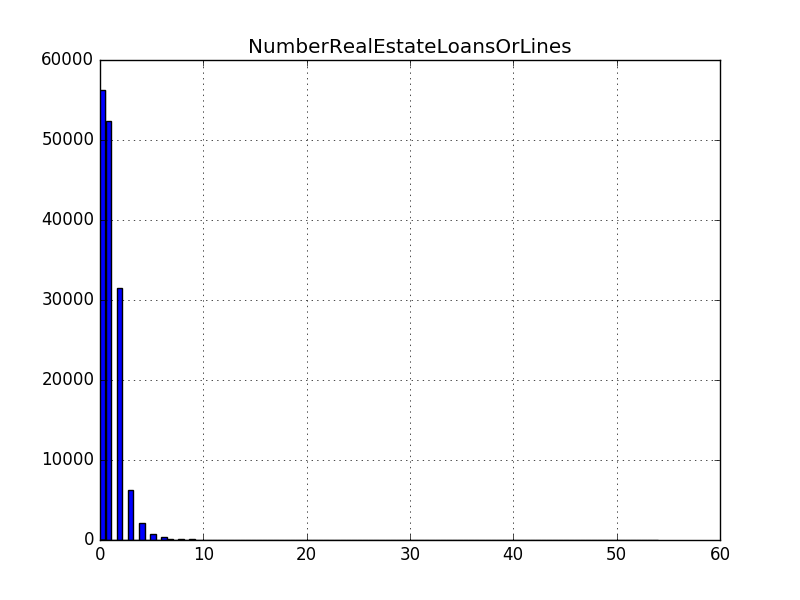
\includegraphics[width=.7\textwidth]{../graphics/train_set_NumberRealEstateLoansOrLines.png}\
\\
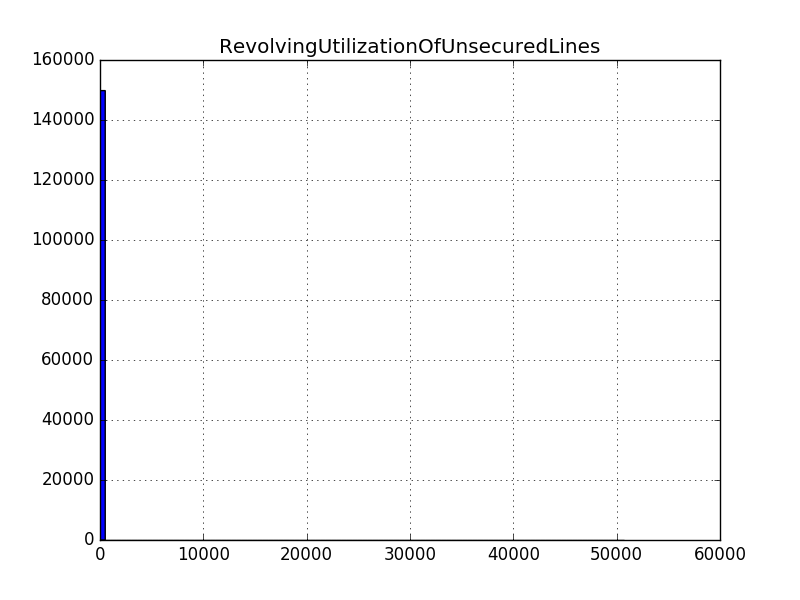
\includegraphics[width=.7\textwidth]{../graphics/train_set_RevolvingUtilizationOfUnsecuredLines.png}
\\
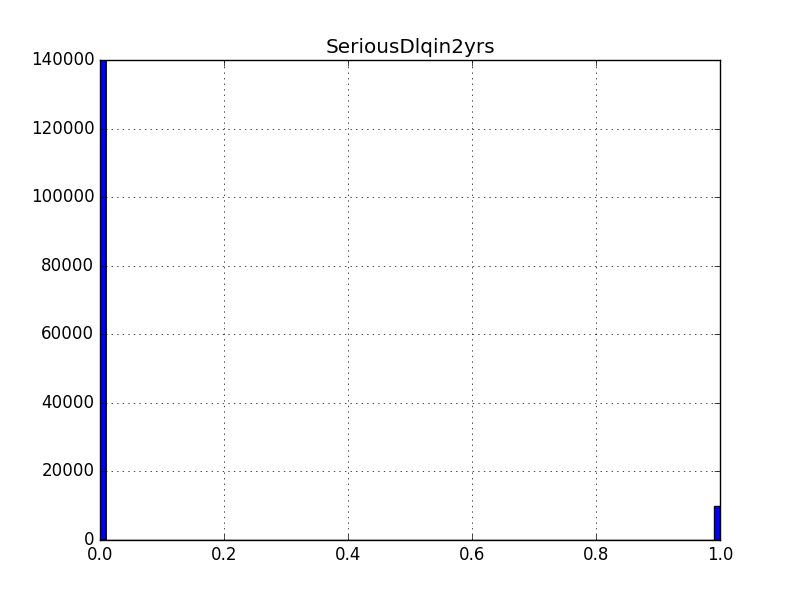
\includegraphics[width=.7\textwidth]{../graphics/train_set_SeriousDlqin2yrs.png}
\\
\end{center}
\newpage
As we can see, a number of the distributions demonstrate extremely long right tails: most of the data is concentrated at low values, but some are at very high values.
\\
Our variable of interest, in the last histogram entitled "SeriousDlqin2Yrs", shows that in the training dataset most of the individuals demonstrated no serious delinquency, but that a small subset showed very high delinquency rates.
\\
\section{Data Imputation}
All of the variables in the dataset are numeric. In order to impute missing values, I simply filled the values the missing values with the mean for that variable. This did not seem like an unreasonable choice given the size of the dataset and the continuous rather than the discrete nature of the variables (in which case mean values more sensitive to categorical regularities might have been used).
\\
This dataset with filled values is included in the repository "predicted
\section{Model Choice and Predicted Values}
In order to predict the values I tried three different machine learning methods \footnote{The three classifiers attempted were K-Nearest Neighbours, Logistic Regression, and Linear SVC}. The best method, called the K-Nearest Neighbors Method (which tries to decide on an unknown type by looking at those what who are most similar on a range of characteristics), which resulted in an accuracy of .934. Unfortunately, this accuracy is not very different from simply assuming all of the borrowers are \emph{NOT} delinquent. In our predicted values (found in the folder "data\_output/predicted\_values.txt") for the test dataset, only one or two borrowers were predicted to be delinquent. In the future, I hope to improve upon this accuracy metric by trying a wider variety of models and model specifics.
\\
The choice of a nearest neighbours method rather than a more probabilities focused logistic regression method seems reasonable because the dataset demonstrates that in probability all individuals will not be delinquent, but broad similarity between individuals across all characteristics may predict risk well.
\end{document}